\documentclass[../main.tex]{subfiles}
% !TeX root = ../main.tex
\begin{document}
	\section{Receivables}
	
	\subsection{Pros and Cons of Extending Credit}
	
	The advantage of extending credit is that it helps customers buy products 
	and services, thereby increasing the seller’s revenues. 
	
	The disadvantages of extending credit are the following additional costs 
	introduced:
	\begin{itemize}[noitemsep]
		\item Increased wage costs. If credit is extended, the company will 
		have to hire people to 
		\begin{itemize}[noitemsep]
			\item evaluate whether each customer is 
			creditworthy
			\item track how much each customer owes
			\item follow up to collect the receivable from each customer.
		\end{itemize}
		\item Bad debt costs. Inevitably, some customers dispute what they owe 
		,or they run into financial difficulties and cannot pay their account 
		balances. These bad debt costs are considered an additional cost of 
		extending credit.
		\item Delayed receipt of cash. Even if the company were to collect in 
		full from customers, it will likely have to wait 30–60 days before 
		receiving the cash.
	\end{itemize}
	
	\subsection{Accounts Receivable}
	
	A \textbf{receivable} is an amount due from another party. The two most 
	common receivables are Accounts Receivable and Notes Receivable. Other 
	receivables include Interest Receivable, Rent Receivable, Tax Refund 
	Receivable, and receivables from employees. Accounts receivable are amounts 
	due from customers for credit sales.
	
	Credit sales are recorded by increasing (debiting) Accounts Receivable. A 
	company must also maintain a separate account for each customer that tracks 
	how much that customer purchases, has already paid, and still owes. This 
	information provides the basis for sending bills to customers and for other 
	business analyses. 
	
	The general ledger continues to have a single Accounts 
	Receivable account along with the other financial statement accounts, but a 
	supplementary record is created to maintain a separate account for each 
	customer. This supplementary record is called the \textbf{accounts 
	receivable 
	ledger}.
	
	\subsubsection{Sales on Credit}

	The credit sale is posted with both a debit to the Accounts Receivable 
	1account in the general ledger and a debit to Accounts Receivable—CompStore 
	customer account in the accounts receivable ledger. 

	The cash receipt from RDA Electronics is posted as a credit to the Accounts 
	Receivable account in the general ledger and to the Accounts Receivable—RDA 
	Electronics customer account in the accounts receivable ledger. 
	
	\begin{figure}[ht]
		\centering
		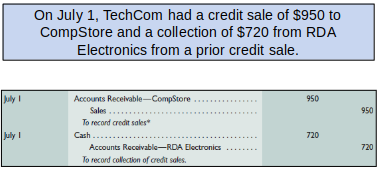
\includegraphics[width=\columnwidth]{images/c6/sales_on_credit_eg.png}
	\end{figure}

	Posting debits or credits to Accounts Receivable in two separate ledgers 
	does not violate the requirement that debits equal credits. The equality of 
	debits and credits is maintained in the general ledger. The accounts 
	receivable ledger is a supplementary record providing information on each 
	customer.
	
	\subsubsection{Credit Card Sales}
	
	Many companies allow their customers to pay for products and services using 
	third-party credit cards such as Visa, MasterCard, or American Express, and 
	debit cards (also called ATM or bank cards). The seller pays a fee for 
	services provided by the card company, often ranging from 1\% to 5\% of 
	card sales. This charge is deducted from the credit to the seller’s account 
	or the cash payment to the seller.
	
	There are several reasons why sellers allow customers to use third-party 
	credit cards and debit cards instead of granting credit directly to 
	customers. 
	\begin{itemize}[noitemsep]
		\item The seller does not have to evaluate each customer’s 
		credit standing or make decisions about who gets credit and how much.
		\item The seller avoids the risk of extending credit to customers who 
		cannot or do not pay. This risk is transferred to the card company.
		\item The seller typically receives cash from the card company sooner 
		than had it granted credit directly to customers.
		\item A variety of credit options 
		for customers offers a potential increase in sales volume.
	\end{itemize}
	
	\begin{figure}[ht]
		\centering
		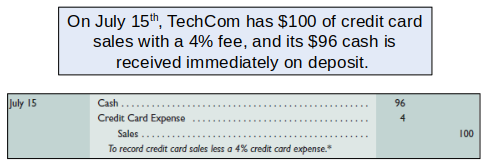
\includegraphics[width=\columnwidth]{images/c6/credit_card_eg.png}
		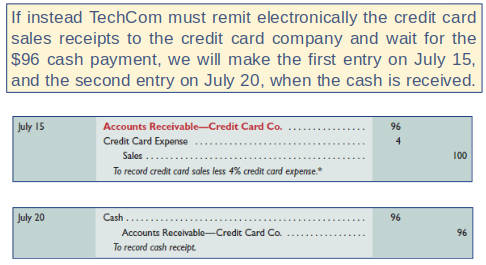
\includegraphics[width=\columnwidth]{images/c6/credit_card_eg2.png}
	\end{figure}
	
	\subsection{Valuing Accounts Receivable}
	
	When a company directly grants credit to its customers, it expects that 
	some customers will not pay what they promised. The accounts of these 
	customers are uncollectible accounts, commonly called \textbf{bad debts}. 
	The total amount of uncollectible accounts is an expense of selling on 
	credit. Companies use two methods to account for uncollectible accounts: 
	\begin{itemize}[noitemsep]
		\item \textbf{Direct write-off method}
		\item \textbf{Allowance method}
	\end{itemize}
	
	\subsubsection{Direct Write-off Method}
	
	The direct write-off method does not estimate bad debt. Instead, it 
	reports Sales when they occur and bad debt expense when it is discovered. 
	This method is not acceptable by GAAP.
	
	\begin{figure}[ht]
		\centering
		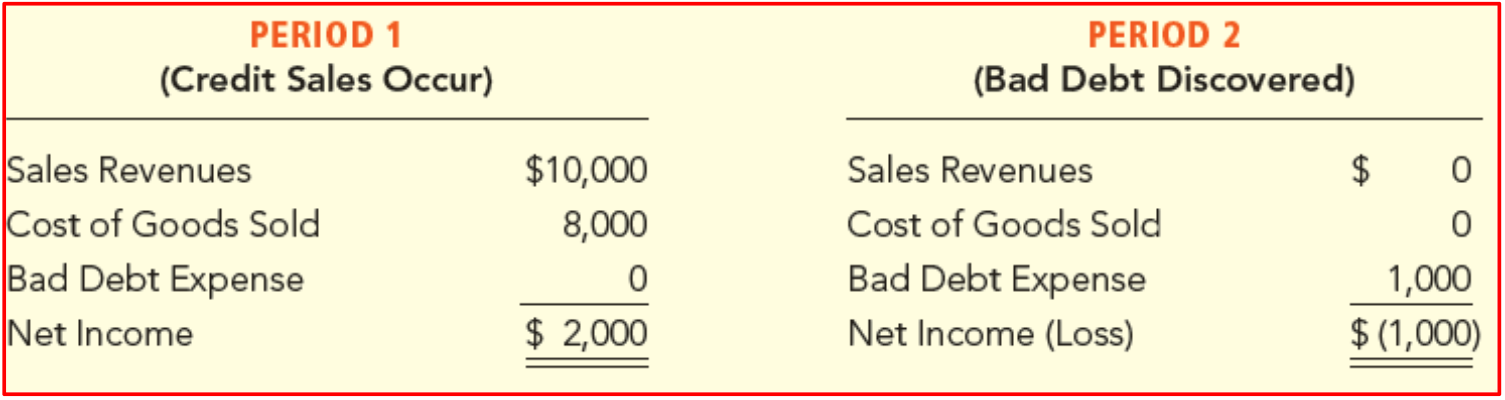
\includegraphics[width=\columnwidth]{images/c6/direct_writeoff.png}
	\end{figure}

	The reason why the method isn't GAAP is because it reports receivables at 
	the total amount owed by customers rather than what is estimated to be 
	collectible and it violates the expense recognition principle (matching 
	principle) by recording bad debt expense in the period when customer's 
	account is determined to be bad rather than the period when the credit 
	sales are actually made. 
	
	When using the direct write-off method, customers’ accounts receivable are 
	written off to Bad Debts Expense at the time the company becomes aware that 
	the customer will not be able to pay the amounts owed.
	
	\begin{figure}[ht]
		\centering
		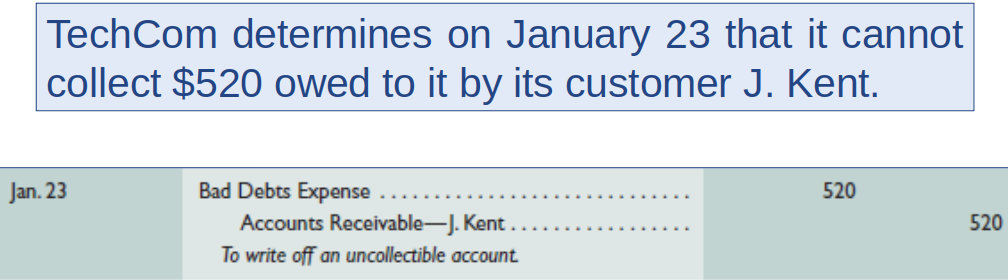
\includegraphics[width=\columnwidth]{images/c6/direct_writeoff_eg.png}
	\end{figure}

	Notice that the specific customer is noted in the transaction so we can 
	make the proper entry in the customer’s Accounts Receivable subsidiary 
	ledger. 

	Now assume that on March 11, J. Kent sends TechCom full payment of \$520 
	after TechCom made the write-off entry. Since TechCom had written off 
	Kent’s account receivable, the first required entry reverses the write-off 
	and re-establishes part of Kent’s account receivable. 
	
	\begin{figure}[ht]
		\centering
		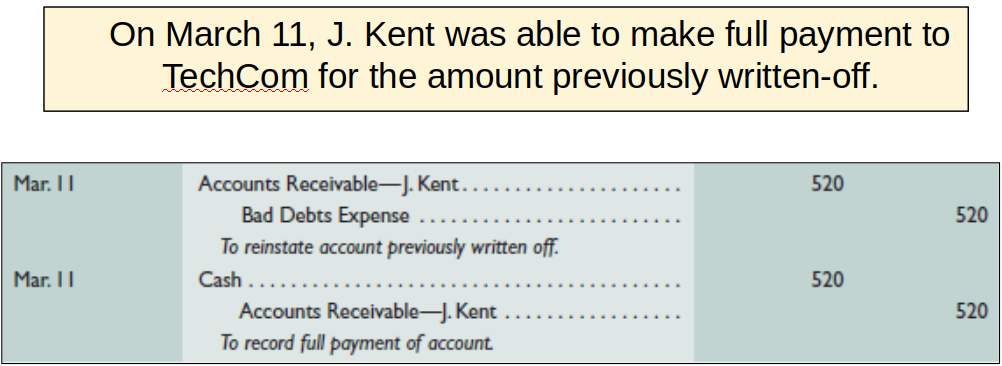
\includegraphics[width=\columnwidth]{images/c6/direct_writeoff_recovery.png}
		\caption{Recovering Bad Debt in Direct Write-Off Method}
	\end{figure}
	
	This entry includes a debit to Accounts Receivable and a credit to Bad 
	Debts Expense. The second entry is a debit to Cash and a credit to Accounts 
	Receivable for the amount of cash received.  

	\subsubsection{Allowance Method}
	
	When a company sells goods or services on account, it records both Accounts 
	Receivable and Sales Revenue. Accounts Receivable is an asset on the 
	balance sheet and Sales Revenue is a revenue account on the income 
	statement. 
	
	Unfortunately, some accounts receivable will never be collected in full, 
	resulting in a bad debt. These bad debts mean that not all accounts 
	receivable will be converted to cash and not all sales will generate 
	profit. Thus, when accounting for accounts receivable and bad debts, there 
	are two objectives:
	\begin{itemize}[noitemsep]
		\item Report accounts receivable at the amount the company expects to 
		collect (“\textbf{net realizable value}”).
		\item Match the estimated cost of bad debts to the accounting period in 
		which the related credit sales are made.
	\end{itemize}
	
	These two objectives point to the same solution: reduce both Accounts 
	Receivable and Net Income by the amount of credit sales that are unlikely 
	to be collected as Cash. To achieve these two objectives, we use the 
	Allowance Method of accounting for bad debts. This method involves 
	subtracting an Allowance for Doubtful Accounts from Accounts Receivable and 
	subtracting Bad Debt Expense when determining Net Income. These amounts are 
	estimated and recorded using an adjusting journal entry at the end of each 
	accounting period in which credit sales are made. 
	
	The adjusting journal entry debits Bad Debt Expense, resulting in an 
	expense on the income statement, and credits Allowance for Doubtful 
	Accounts, resulting in a contra-asset on the balance sheet. 
	
	\begin{figure}[ht]
		\centering
		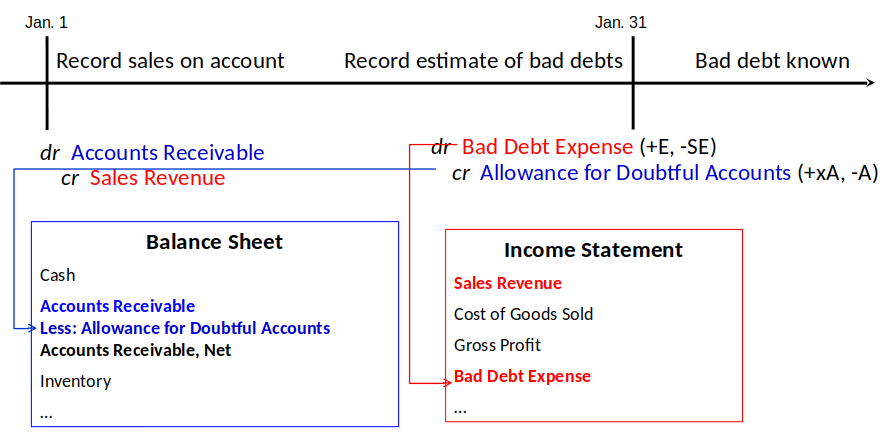
\includegraphics[width=\columnwidth]{images/c6/allowance_method.png}
		\caption{Allowance Method}
	\end{figure}
	
	The first step in the Allowance Method, which is to record an estimate of 
	bad debts in the period sales are made on account. The final step in the 
	Allowance Method occurs when a customer account is finally known to be 
	uncollectible. At this point, a journal entry is recorded to remove the 
	customer’s balance from Accounts Receivable and to remove the same amount 
	from the Allowance for Doubtful Accounts. This final step is known as 
	\textbf{writing-off the customer’s account}.
	
	Notice that this journal entry does not involve Bad Debt Expense. That 
	expense was already recorded, in the period that the credit sale initially 
	occurred. The entry to write-off an account when it is known to be 
	uncollectible has no effect on the income statement. It has little effect 
	on the balance sheet because the reduction in the asset Accounts Receivable 
	is offset by the reduction in the contra-asset Allowance for Doubtful 
	Accounts.  
	
	The allowance method follows a two-step process:
	\begin{enumerate}[noitemsep]
		\item Make an end-of-period adjustment to record the estimated bad 
		debts in the period credit sales occur. 
		\item Remove ('write-off') specific customer balances when they are 
		known to be uncollectible. 
	\end{enumerate}
	
	The allowance method of accounting for bad debts matches the estimated loss 
	from uncollectible accounts receivable against the sales they helped 
	produce. We must use estimated losses because when sales occur, management 
	does not know which customers will not pay their bills. 
	
	This means that at 
	the end of each period, the allowance method requires an estimate of the 
	total bad debts expected to result from that period’s sales. This method 
	has two advantages over the direct write-off method because it: 
	\begin{itemize}[noitemsep]
		\item Records estimated bad debts expense in the period when the 
		related sales are recorded, and 
		\item Reports accounts receivable on the statement of financial 
		position at the estimated amount of cash to be collected.
	\end{itemize}
	
	\begin{figure}[ht]
		\centering
		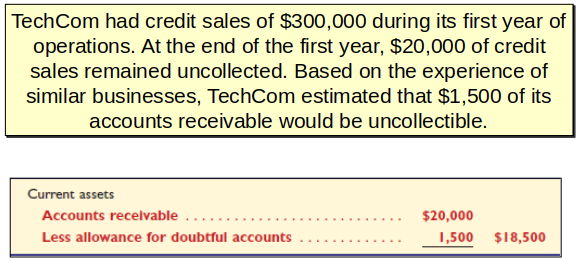
\includegraphics[width=\columnwidth]{images/c6/allowance_sfp.png}
		\caption{Allowance Method: Statement of Financial Position Presentation}
		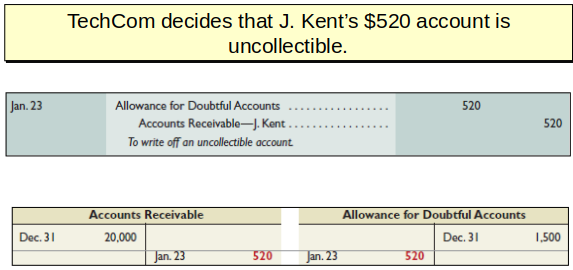
\includegraphics[width=\columnwidth]{images/c6/allowance_writeoff.png}
		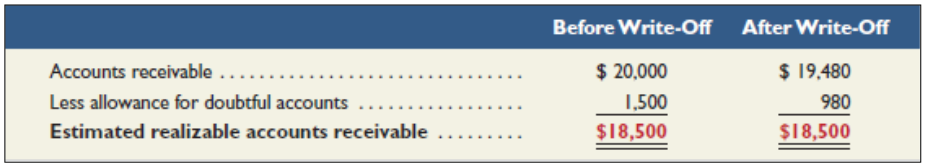
\includegraphics[width=\columnwidth]{images/c6/allowance_writeoff_result.png}
		\caption{Allowance Method: Writing Off a Bad Debt}
	\end{figure}
	
	The write-off does not affect the realizable value of accounts receivable 
	as shown on this slide. Neither total assets nor net profit is affected by 
	the write-off of a specific account. Instead, both assets and net profit 
	are affected in the period when bad debts expense is predicted and recorded 
	with an adjusting entry. 
	
	When a customer fails to pay and the account is written off as 
	uncollectible, his or her credit standing is jeopardized. To help restore 
	credit standing, a customer sometimes volunteers to pay all or part of the 
	amount owed. 
	
	\begin{figure}[ht]
		\centering
		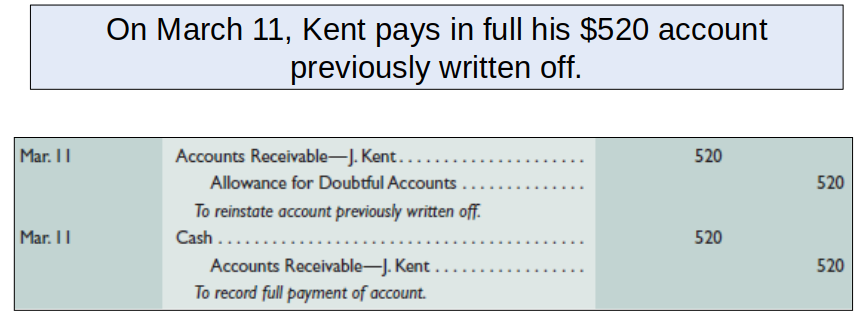
\includegraphics[width=\columnwidth]{images/c6/allowance_recovery.png}
		\caption{Allowance Method: Recovering a Bad Debt}
	\end{figure}
	
	A company makes two entries when collecting an account 
	previously written off by the allowance method. The first is to reverse the 
	write-off and reinstate the customer’s account. The second entry records 
	the collection of the reinstated account.
	
	\subsection{Methods for Estimating Bad Debt}
	
	There are two methods of estimating bad debts in a given period:
	\begin{itemize}[noitemsep]
		\item \textbf{Percentage of Receivables method} 
		\item \textbf{Aging of Receivables method} 
	\end{itemize}
	Both methods are acceptable under GAAP and IFRS. The percentage of credit 
	sales method is simpler to apply, but the aging method uses more detailed 
	data and therefore is generally more accurate. Some companies use the 
	simpler method on a weekly or monthly basis and the more accurate method on 
	a monthly or quarterly basis to check the accuracy of earlier estimates.
	
	\subsubsection{Percent of Receivables Method}
	
	When using the Percent of Receivables Method, the estimate at the end of 
	the period is determined by taking the Accounts Receivable balance and 
	multiplying by an established bad debt percentage. 
	\[
	\text{Year-end Accounts Receivable} \times \text { Bad Debt } \%
	\]
	The bad debt percentage 
	is determined based on past history of the company and current economic 
	trends. This computation provides the company with the balance desired in 
	the Allowance for Doubtful Accounts. 
	
	Because the Allowance for Doubtful Accounts is a permanent account, it will 
	always have a balance in it.  As a result, when we determine the desired 
	balance in step one, we have to then look and see what balance is already 
	in the Allowance for Doubtful Accounts and make the entry for the amount 
	needed to arrive at the desired balance.
	\[
	\text{Bad Debts Expense} = \text{Estimated Receivable} - \text{Previous 
	Balance}
	\]
	
	\begin{figure}[ht]
		\centering
		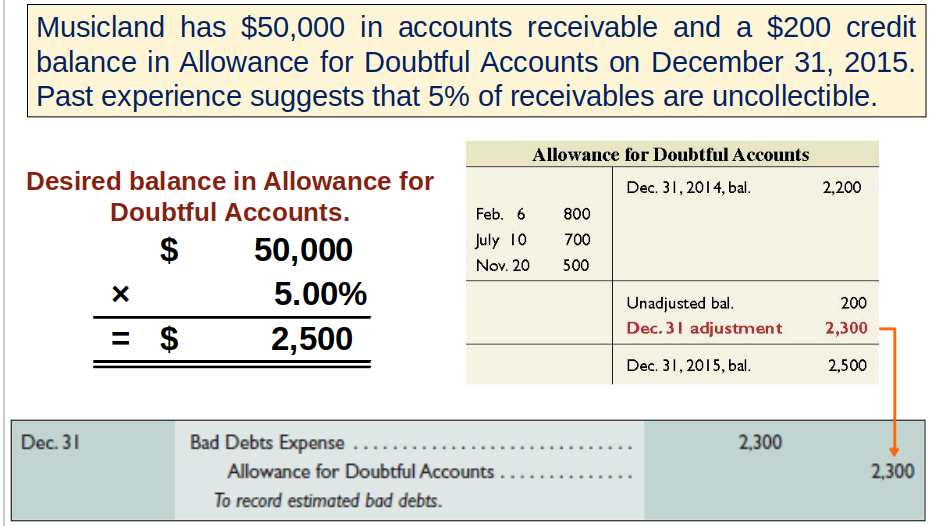
\includegraphics[width=\columnwidth]{images/c6/percent_receivables_eg.png}
	\end{figure}
	
	\subsubsection{Aging of Receivables Method}
	
	The aging method gets its name because it is based on the 'age' of each 
	amount in Accounts Receivable at the end of the period. The older and more 
	overdue an account receivable becomes, the less likely it is to be 
	collectible. 
	
	 This method uses both past and current receivables information to estimate 
	 the allowance amount. Specifically, each receivable is classified by how 
	 long it is past its due date. Then estimates of uncollectible amounts are 
	 made assuming that the longer an amount is past due, the more likely it is 
	 to be uncollectible. 
	 
	 Classifications are often based on 30-day periods. 
	 After the amounts are classified (or aged), experience is used to estimate 
	 the percent of each uncollectible class. These percents are applied to the 
	 amounts in each class and then totaled to get the estimated balance of the 
	 Allowance for Doubtful Accounts.
	 
	 This method works by:
	 \begin{enumerate}[noitemsep]
	 	\item Classify each receivable by how long it is past due.
	 	\item Each age group is multiplied by its estimated bad debt percentage.
	 	\item Estimated bad debts for each group are totaled.
	 \end{enumerate}
	
	\begin{figure}[ht]
		\centering
		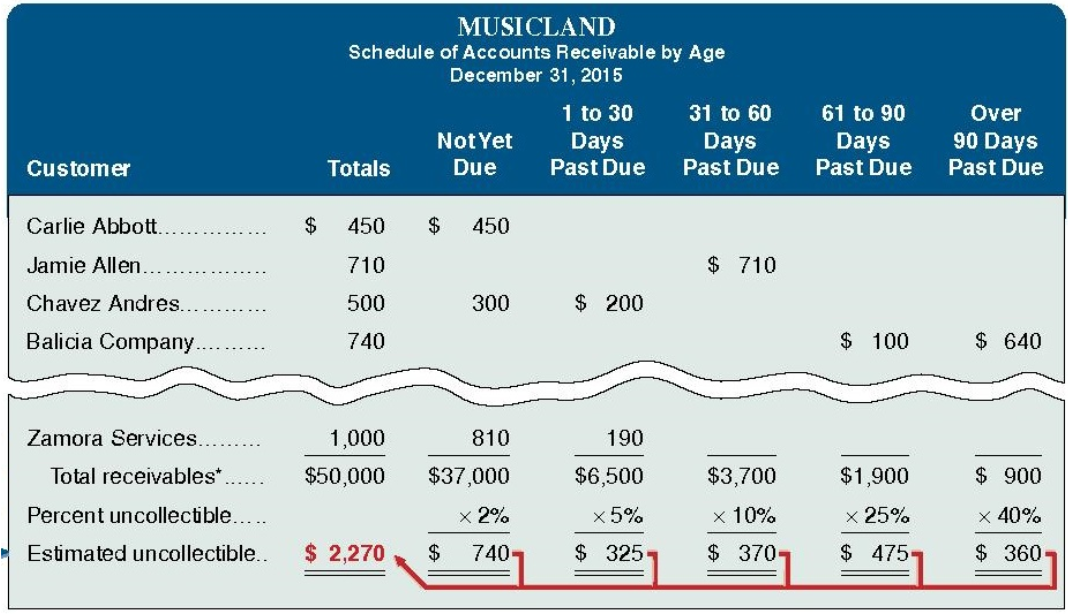
\includegraphics[width=\columnwidth]{images/c6/aging_receivables_eg.png}
		\caption{This aging of accounts lists each customer’s individual 
		balances assigned to one of five classes based on its days past due. 
		The amounts in each class are totaled and multiplied by the estimated 
		percent of uncollectible accounts for each class. The percents used are 
		regularly reviewed to reflect changes in the company and economy.}
	\end{figure}
	
	
	\begin{figure}[ht]
		\centering
		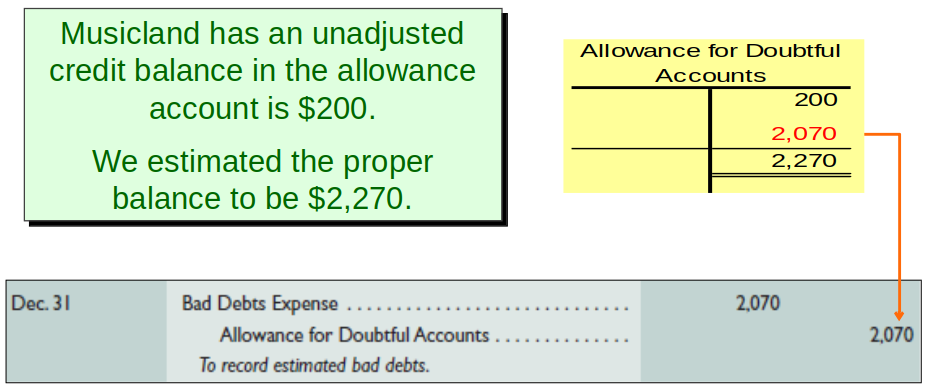
\includegraphics[width=\columnwidth]{images/c6/aging_eg2.png}
	\end{figure}
	
	Total Accounts Receivable written off during a period will rarely equal the 
	estimated allowance. The allowance account will show a debit balance when 
	the total amount of accounts receivable written off is greater than the 
	estimated allowance.  It needs to be adjusted to become a credit balance 
	before preparing the financial statements. The allowance account will show 
	a credit balance when the total amount of accounts receivable written off 
	is less than the estimated allowance. This is the normal balance for this 
	account.
	
	\subsubsection{Individual and Group Estimation of Bad Debts}
	
	As stated in IAS 39, assessment of impairment losses for financial assets 
	can be categorized into three types:
	\begin{itemize}[noitemsep]
	\item Assessment at “individual” asset level for all individually 
	significant 
	items.
	\item For individually non-significant items, the entity has a choice 
	either 
	to assess it individually or collectively for a group of assets with 
	similar credit risk features.
	\item Collective assessment of impairment for items where no individual 
	impairment exists but forms part of a group of assets with similar credit 
	characteristics.
	\end{itemize}
	
	\subsection{Notes Receivable and Interest Revenue}
	
	A company reports Notes Receivable if it uses a \textbf{promissory note} to 
	document its right to collect money from another party. This usually 
	happens in the following three situations:
	\begin{itemize}[noitemsep]
		\item the company loans money to employees or businesses,
		\item the company sells expensive items for which customers require an 
		extended payment period, or
		\item the company converts an existing account receivable to a note 
		receivable to allow an extended payment period.
	\end{itemize}
	
	A \textbf{promissory note} is a written promise to pay a specified amount 
	of money, usually with interest, either on demand or at a definite future 
	date. To a borrower, interest is an expense. To a lender, it is revenue. 
	Promissory notes are used in many transactions, including paying for 
	products and services, and lending and borrowing money. Sellers sometimes 
	ask for a note to replace an account receivable when a customer requests 
	additional time to pay a past-due account. 
	
	\begin{figure}[ht]
		\centering
		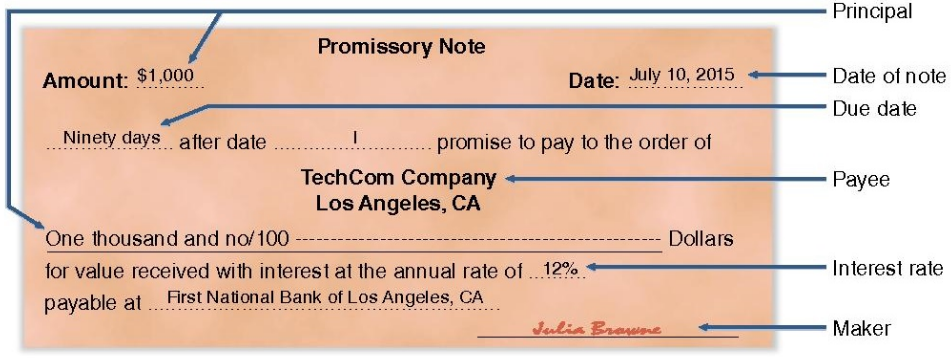
\includegraphics[width=\columnwidth]{images/c6/promissory_note.png}
		\caption{Promissory Note}
	\end{figure}
	
	For legal reasons, sellers 
	generally prefer to receive notes when the credit period is long and when 
	the receivable is for a large amount. If a lawsuit is needed to collect 
	from a customer, a note is the buyer’s written acknowledgment of the debt, 
	its amount, and its terms.
	
	\subsubsection{Maturity}
	
	The \textbf{maturity date of a note} is the day the note (principal and 
	interest) 
	must be repaid. The \textbf{period of a note} is the time from the note’s 
	(contract) 
	date to its maturity date. Many notes mature in less than a full year, and 
	the period they cover is often expressed in days. When the time of a note 
	is expressed in days, its maturity date is the specified number of days 
	after the note’s date. 
	
	\begin{figure}[ht]
		\centering
		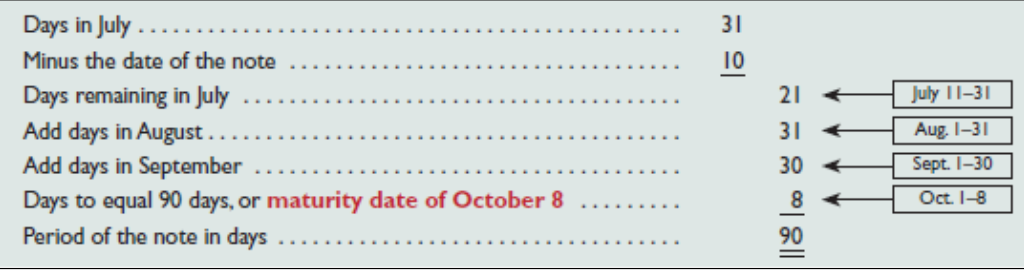
\includegraphics[width=\columnwidth]{images/c6/notes_receivable_example.png}
		\caption{Promissory Note Example. This note is due and payable on 
		October 8, 2015}
	\end{figure}

	\subsubsection{Interest Computation}
	
	Interest is the cost of borrowing.  It is calculated as Principal times 
	Rate times Time. Remember that interest rates are reported for a year. 
	
	\begin{figure}[ht]
		\centering
		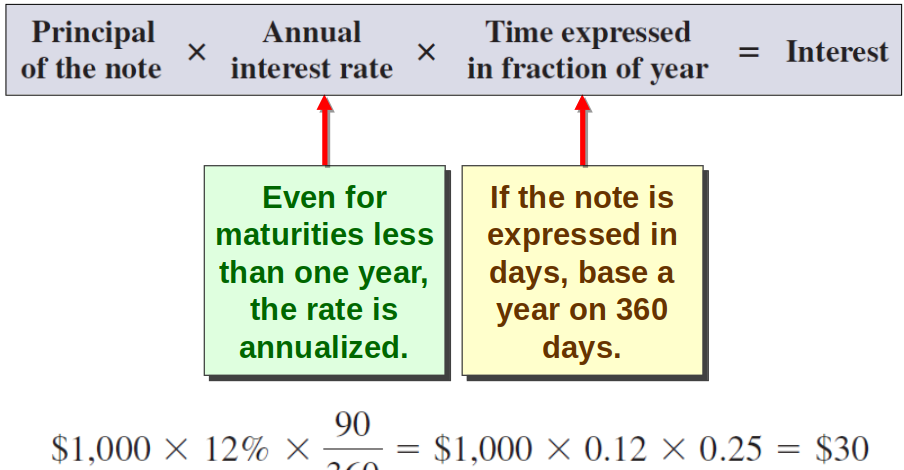
\includegraphics[width=0.8\columnwidth]{images/c6/interest_computation.png}
	\end{figure}
	So, if we just took Principal times Rate, we would get the interest for an 
	entire year. We need to continue to multiply by Time to get the interest 
	for the portion of the year the note was outstanding. Remember that 
	accountants use a year based on 360 days rather than 365 days.
	
	\subsubsection{Recognizing Notes Receivable}
	
	Notes receivable are usually recorded in a single Notes Receivable account 
	to simplify recordkeeping. The original notes are kept on file, including 
	information on the maker, rate of interest, and due date. (When a company 
	holds a large number of notes, it sometimes sets up a controlling account 
	and a subsidiary ledger for notes. This is similar to the handling of 
	Accounts Receivable.) 
	
	\begin{figure}[ht]
		\centering
		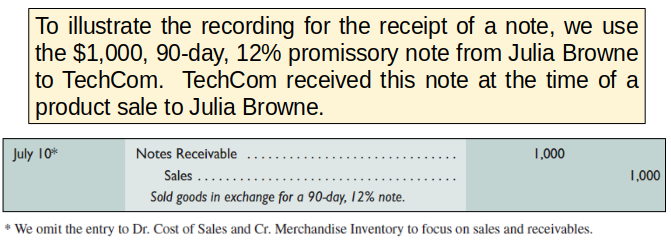
\includegraphics[width=1\columnwidth]{images/c6/notes_receivable_eg.png}
		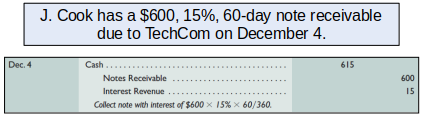
\includegraphics[width=1\columnwidth]{images/c6/honored_note_eg.png}
		\caption{Recording an Honored Note}
		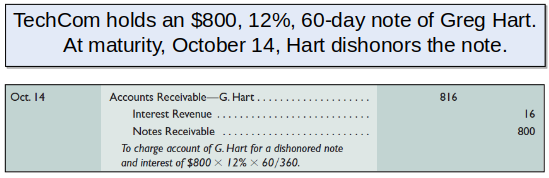
\includegraphics[width=1\columnwidth]{images/c6/dishonored_note_eg.png}
		\caption{Recording a Dishonored Note}
	\end{figure}
	
	When a note’s maker is unable or refuses to pay at maturity, the note is 
	dishonored. The act of dishonoring a note does not relieve the maker of the 
	obligation to repay the principal and interest due.
	
	\subsubsection{Recording End-of-Period Interest Adjustments}
	
	\begin{figure}[ht!]
		\centering
		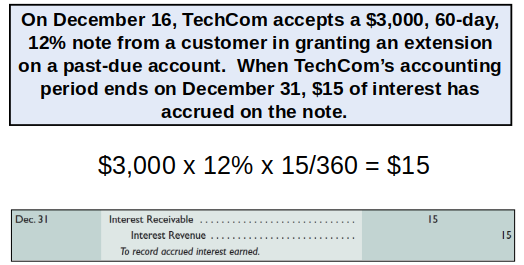
\includegraphics[width=.8\columnwidth]{images/c6/interest_adjustments_eg.png}
		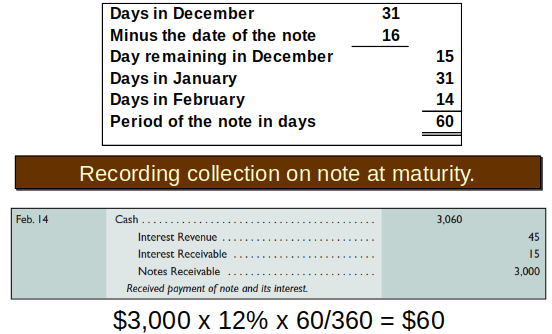
\includegraphics[width=.8\columnwidth]{images/c6/interest_collection_eg2.png}
	\end{figure}
	
\end{document}